\def\detectionbranch{
    nhánh xác định đối tượng\index{nhánh xác định đối tượng} của RetinaFocus được xây dựng dựa trên mô hình RetinaFace \cite{deng2020retinaface}, một mô hình một pha\index{một pha} giải quyết bài toán nhận diện khuôn mặt đạt kết quả tốt trên bộ dữ liệu WIDER FACE \cite{yang2016wider}.

    \noindent
    nhánh xác định đối tượng\index{nhánh xác định đối tượng} cũng sử dụng kiến trúc FPN nhằm trích xuất đặc trưng của ảnh đầu vào với nhiều kích thước bản đồ đặc trưng\index{bản đồ đặc trưng} khác nhau.
    Tuy nhiên, tương tự như RetinaFace \cite{deng2020retinaface}, nhánh xác định đối tượng\index{nhánh xác định đối tượng} đưa các bản đồ đặc trưng\index{bản đồ đặc trưng} này qua các Context Module \cite{najibi2017ssh} nhằm thu thập thêm các thông tin về background\index{background} xung quanh trước khi đưa ra dự đoán về hộp giới hạn\index{hộp giới hạn} chứa khuôn mặt.
    Ý tưởng sử dụng các khối Context Module \cite{najibi2017ssh} tỏ ra khá hiệu quả khi áp dụng với bài toán nhận diện khuôn mặt.
    Đặc biệt trong việc định vị các mặt nhỏ, vì khi những thông tin về background\index{background} xung quanh như thân người sẽ có vai trò quan trọng giúp mô hình học tốt hơn.
    Trong kiến trúc của nhánh xác định đối tượng\index{nhánh xác định đối tượng}, ba bản đồ đặc trưng\index{bản đồ đặc trưng} \textit{{${P}_{3}, {P}_{4}, {P}_{5}$}} của FPN của mô hình xương sống được đưa qua ba khối Context Module độc lập.
    Mỗi khối Context Module gồm ba khối Conv nối tiếp nhau, nhưng bản đồ đặc trưng\index{bản đồ đặc trưng} đầu ra của mỗi khối Conv đều được concat lại với nhau để tạo ra bản đồ đặc trưng\index{bản đồ đặc trưng} cuối cùng của cả khối Context Module.

    \noindent
    Đầu ra nhánh xác định đối tượng\index{nhánh xác định đối tượng} của RetinaFocus gồm toạ độ của hộp giới hạn\index{hộp giới hạn} dự đoán của mô hình, toạ độ của landmarks của khuôn mặt và xác suất mà hộp giới hạn\index{hộp giới hạn} dự đoán đó chứa khuôn mặt.
    Các đầu ra này tiếp tục được đưa vào hàm mất mát đa nhiệm vụ\index{hàm mất mát đa nhiệm vụ}, tương tự như mô hình RetinaFace.

    \begin{figure}[H]
        \centering
        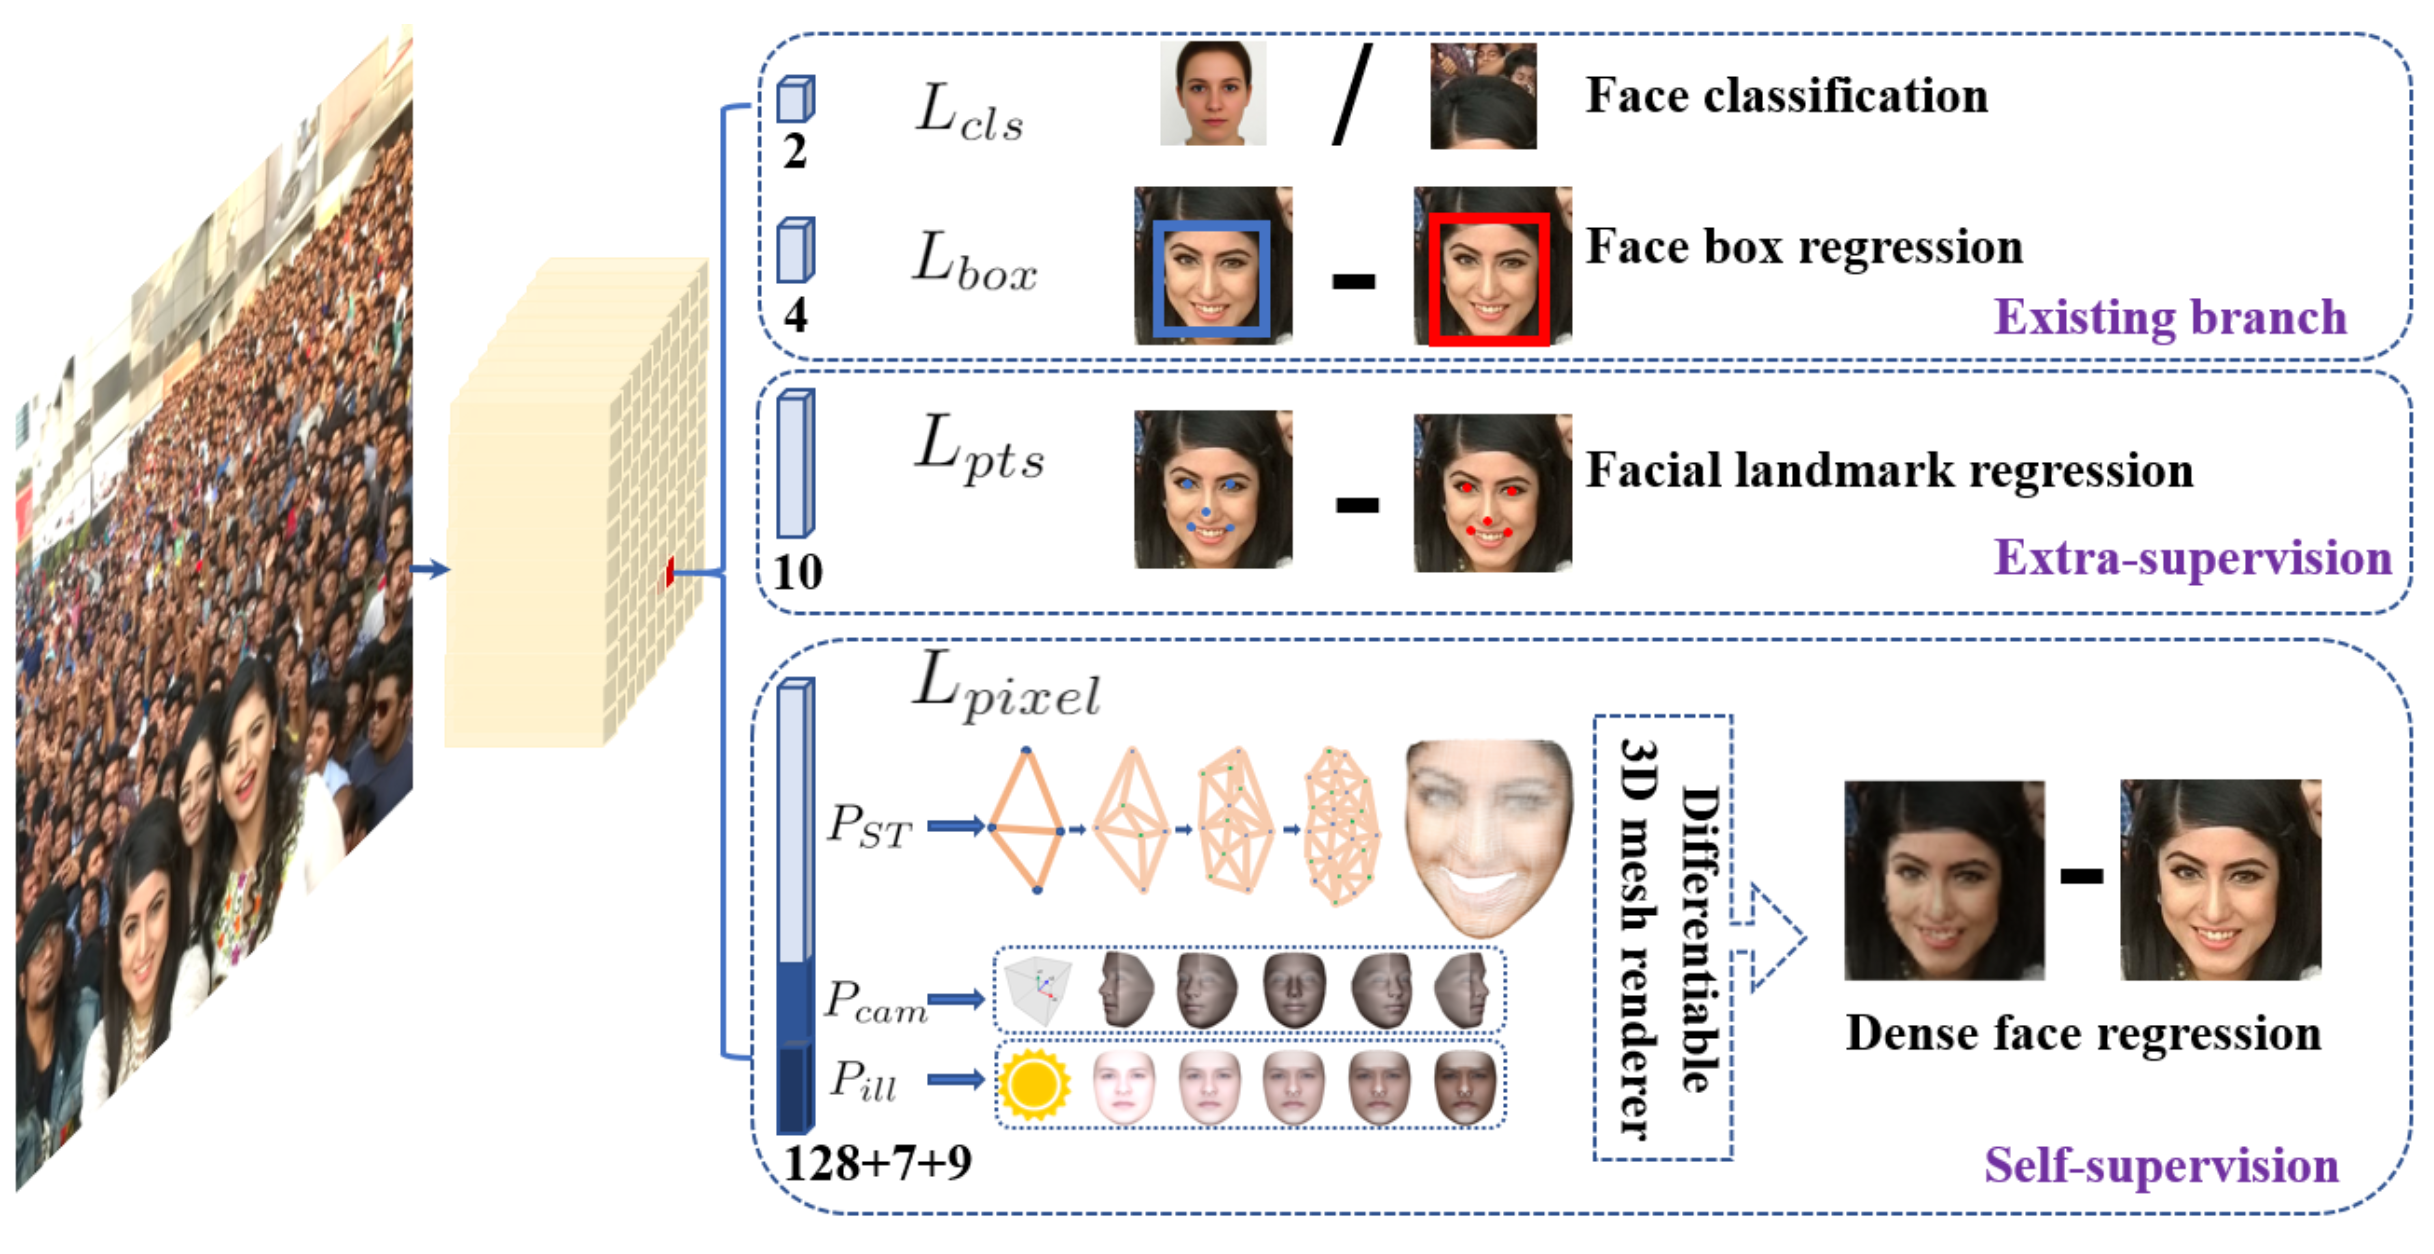
\includegraphics[width=10cm] {images/retinaface_loss_funcs}
        \caption{Ý tưởng các hàm mất mát đa nhiệm vụ\index{hàm mất mát đa nhiệm vụ} của mô hình RetinaFace. Ngoài hàm mất mát tự giám sát \cite{zhou2019dense, genova2018unsupervised}, các hàm mất mát còn lại được kế thừa cho mô hình RetinaFocus (Nguồn: \cite{deng2020retinaface})}
        \label{fig:retinaface_loss_funcs}
    \end{figure}

    \noindent
    Cụ thể, trong quá trình huấn luyện mô hình, với mỗi khu vực mỏ neo\index{khu vực mỏ neo}, nhánh xác định đối tượng\index{nhánh xác định đối tượng} của mô hình RetinaFocus tối ưu hàm mất mát đa nhiệm vụ\index{hàm mất mát đa nhiệm vụ} dưới đây:

    \begin{equation}
        \begin{split}
        L  & =  L_{cls}(p_i, p^{*}_i) + \lambda_1 p^{*}_i L_{box}(t_i, t^{*}_i) + \lambda_2 p^{*}_i L_{pts} (l_i, l^{*}_i).\\
        \end{split}
        \label{eq:retinaface_loss}
    \end{equation}

    \noindent
    trong đó: \\
    - Các trọng số $\lambda_1, \lambda_2, \lambda_3$ được cấu hình mặc định là 0.25, 0.1 và 0.01. \\
    - Hàm mất mát phân lớp mặt: \\
    $L_{cls}(p_i, p^{*}_i)$ với $p_i$ là xác suất mà mô hình dự đoán một khu vực mỏ neo\index{khu vực mỏ neo} có chứa là khuôn mặt hay không.
    Ta có $p^{*}_i = 1$ nếu khu vực mỏ neo\index{khu vực mỏ neo} đó chứa khuôn mặt còn $p^{*}_i = 0$ nếu khu vực mỏ neo\index{khu vực mỏ neo} đó không chứa khuôn là mặt. \\
    - Hàm mất mát hồi quy định vị vị trí của bbox: \\
    $L_{box}(t_i, t^{*}_i)$ với $t_i=\{t_x, t_y, t_w, t_h\}_i$ và $t^{*}_i=\{t^{*}_x, t^{*}_y, t^{*}_w, t^{*}_h\}_i$ lần lượt là bộ bốn tham số đại diện cho toạ độ của khu vực mỏ neo\index{khu vực mỏ neo} mà mô hình dự đoán là mặt và bbox groundtruth\index{groundtruth} từ bộ dữ liệu.
    (x là toạ độ x của điểm góc trái trên, y là toạ độ y của điểm góc trái trên, w là chiều rộng của bbox và h là chiều cao của bbox). \\
    - Hàm mất mát hồi quy định vị vị trí của landmarks: \\
    $L_{pts} (l_i, l^{*}_i)$ với $l_i=\{l_{x_1}, l_{y_1}, \dots , l_{x_5}, l_{y_5}\}_i$ và $l^{*}_i=\{l^{*}_{x_1}, l^{*}_{y_1}, \dots , l^{*}_{x_5}, l^{*}_{y_5}\}_i$ lần lượt là bộ mười tham số đại diện cho toạ độ của năm landmarks mà mô hình dự đoán ứng với mỗi hộp giới hạn\index{hộp giới hạn} dự đoán và năm groundtruth\index{groundtruth} landmarks của mỗi groundtruth\index{groundtruth} hộp giới hạn\index{hộp giới hạn} từ bộ dữ liệu.
}